\documentclass[conference]{IEEEtran}
\IEEEoverridecommandlockouts
% The preceding line is only needed to identify funding in the first footnote. If that is unneeded, please comment it out.
\usepackage{cite}
\usepackage{amsmath,amssymb,amsfonts}
\usepackage{algorithmic}
\usepackage{graphicx}
\usepackage{booktabs}
\usepackage{textcomp}
\usepackage{xcolor}
\def\BibTeX{{\rm B\kern-.05em{\sc i\kern-.025em b}\kern-.08em
    T\kern-.1667em\lower.7ex\hbox{E}\kern-.125emX}}
\begin{document}

% =========================================================================
% CATATAN KERJA (hapus blok komentar ini sebelum kirim):
% - Isi [TIM] di Seksi II-A (tanggal pencarian Scopus) dan [ISI TANGGAL]
%   pada keterangan Gambar 1.
% - [FULLTEXT-VERIFY] di Seksi IV-C: cek angka CR 0,046 dari [8] saat PDF ada.
% - Gambar 1 sudah terhubung ke prisma-diagram.png (render 2x dari
%   prisma-diagram.svg, angka sudah 109). Jika butuh vektor, konversi
%   SVG ke PDF lalu ganti ekstensi di \includegraphics.
% - Judul run-in bawaan IEEEtran: "Abstract---" dan "Index Terms---";
%   jika dosen minta bahasa Indonesia, ubah dengan \renewcommand.
% - HAPUS komentar template merah bawaan di bawah sebelum submit.
% =========================================================================

\title{Decision Support Systems for Urban Surveillance and Public Safety Facility Placement: A Scoping Review and Conceptual Framework for CCTV Prioritization in Jatinangor Student Settlements}

\author{\IEEEauthorblockN{1\textsuperscript{st} Nama Mahasiswa A}
\IEEEauthorblockA{\textit{Program Studi Decision Support System} \\
\textit{Universitas Padjadjaran}\\
Jatinangor, Indonesia \\
nama.a@mail.unpad.ac.id}
\and
\IEEEauthorblockN{2\textsuperscript{nd} Nama Mahasiswa B}
\IEEEauthorblockA{\textit{Program Studi Decision Support System} \\
\textit{Universitas Padjadjaran}\\
Jatinangor, Indonesia \\
nama.b@mail.unpad.ac.id}
\and
\IEEEauthorblockN{3\textsuperscript{rd} Nama Mahasiswa C}
\IEEEauthorblockA{\textit{Program Studi Decision Support System} \\
\textit{Universitas Padjadjaran}\\
Jatinangor, Indonesia \\
nama.c@mail.unpad.ac.id}
\and
\IEEEauthorblockN{4\textsuperscript{th} Nama Mahasiswa D}
\IEEEauthorblockA{\textit{Program Studi Decision Support System} \\
\textit{Universitas Padjadjaran}\\
Jatinangor, Indonesia \\
nama.d@mail.unpad.ac.id}
\and
\IEEEauthorblockN{5\textsuperscript{th} Nama Mahasiswa E}
\IEEEauthorblockA{\textit{Program Studi Decision Support System} \\
\textit{Universitas Padjadjaran}\\
Jatinangor, Indonesia \\
nama.e@mail.unpad.ac.id}
}

\maketitle

\begin{abstract}
Permukiman mahasiswa Jatinangor diwarnai gang sempit, penerangan jalan terbatas, mobilitas malam tinggi, dan penempatan CCTV yang sporadis akibat keterbatasan anggaran, sehingga alokasi fasilitas pengawasan memerlukan prioritisasi yang terukur. Kajian ini memetakan literatur Decision Support System (DSS) untuk urban surveillance dan public safety facility placement melalui scoping review berbasis PRISMA-ScR di database Scopus (TITLE-ABS-KEY; 2021--2026, artikel, bahasa Inggris), dengan alur seleksi 582 rekaman disaring, 416 laporan diminta untuk diambil, 121 laporan dinilai pada tahap teks lengkap, dan 12 studi disertakan. Sintesis menunjukkan lima pola arsitektur DSS (GIS-MCDM, optimasi coverage, expert-driven, simulasi-DSS, dan policy-MCDA), sebaran metode MCDM dengan pola dominan AHP untuk pembobotan dan TOPSIS untuk perankingan, serta taksonomi kriteria benefit, cost, dan context-dependent. Berdasarkan sintesis tersebut, dirumuskan model konseptual DSS untuk Jatinangor berupa alternatif segmen gang (A1--A5), matriks sembilan kriteria keselamatan (C1--C9), skema pembobotan AHP tiga kelompok pemangku kepentingan, dan perankingan TOPSIS yang menghasilkan peta prioritas penempatan CCTV bertahap sesuai anggaran.
\end{abstract}

\begin{IEEEkeywords}
Decision Support System, Multi-Criteria Decision Making, Scoping Review, PRISMA-ScR, AHP, TOPSIS, CCTV placement, Smart Living and Safety, Jatinangor
\end{IEEEkeywords}

\section{PENDAHULUAN}

Kawasan Jatinangor, Kabupaten Sumedang, merupakan kawasan pendidikan tinggi dengan konsentrasi perguruan besar dan ribuan mahasiswa yang menghuni indekos serta rumah susun di sepanjang koridor kampus. Pertumbuhan hunian padat ini tidak diimbangi kapasitas pengawasan lingkungan: gang-gang permukiman sempit, jangkauan Penerangan Jalan Umum (PJU) belum merata, dan mobilitas malam hari tinggi antara kampus, indekos, dan simpul layanan. Kondisi tersebut menempatkan isu keselamatan dan keamanan warga, khususnya mahasiswa, sebagai persoalan Smart Living and Safety yang nyata di Jatinangor.

Fasilitas pengawasan seperti CCTV hanya dapat ditambahkan secara terbatas karena terkendala anggaran, tiang, pasokan listrik, dan jaringan. Penempatan yang sporadis justru menghasilkan blind zone dan investasi yang tidak efisien. Decision Support System (DSS) berbasis Multi-Criteria Decision Making (MCDM) menawarkan jalur yang sesuai: beberapa kriteria dinilai secara simultan untuk menghasilkan skor dan perankingan alternatif, sehingga keputusan alokasi anggaran memiliki dasar yang dapat dipertanggungjawabkan. Dalam literatur, AHP lazim dipakai untuk pembobotan kriteria berbasis penilaian pakar, sedangkan TOPSIS dipakai untuk perankingan alternatif \cite{kanj2024}, dan kombinasi keduanya terbukti bekerja pada data tabular serta penilaian pakar tanpa infrastruktur sensor berbiaya tinggi \cite{baddour2026}.

Kajian ini dibatasi pada domain Smart Living and Safety di kawasan Jatinangor dengan bukti empiris yang tersedia secara lokal (data tabular, spasial statis, dan penilaian pakar), serta pada literatur scoping review terbitan 2021--2026. Melalui pemetaan literatur yang terstruktur, kajian ini dipandu oleh tiga pertanyaan penelitian:

\begin{itemize}
\item \textbf{RQ1 (Pemetaan Arsitektur DSS):} Bagaimana arsitektur DSS Smart Living \& Safety dipetakan dari literatur (alur input data heterogen ke engine MCDM/analitik lalu output keputusan), dan pola mana yang paling transferable terhadap keterbatasan data Jatinangor?
\item \textbf{RQ2 (Sebaran Metode \& Taksonomi Kriteria MCDM):} Metode MCDM apa yang digunakan dalam DSS Smart Living \& Safety, bagaimana skema pembobotan dan perankingannya diterapkan, serta bagaimana kriteria keputusan diklasifikasikan berdasarkan atribut benefit dan cost?
\item \textbf{RQ3 (Formulasi Model Konseptual Jatinangor):} Model konseptual DSS seperti apa yang paling layak diterapkan untuk prioritisasi CCTV di permukiman mahasiswa Jatinangor, mencakup representasi segmen gang sebagai alternatif, struktur sembilan kriteria keselamatan, skema pembobotan AHP multistakeholder dan perankingan TOPSIS, serta elemen literatur apa yang sengaja tidak diadopsi beserta alasannya?
\end{itemize}

Kontribusi kajian ini terhadap jawaban ketiga RQ tersebut adalah sebagai berikut:

\begin{itemize}
\item \textbf{Kontribusi pertama (RQ1):} pemetaan lima pola arsitektur DSS keselamatan perkotaan beserta penanda kebutuhan datanya, sehingga teridentifikasi pola GIS-MCDM dan optimasi coverage sebagai arsitektur paling transferable untuk Jatinangor, sementara pola simulasi-DSS ditolak dengan argumen kebutuhan kalibrasi yang tidak tersedia.
\item \textbf{Kontribusi kedua (RQ2):} taksonomi sebaran metode MCDM (peran pembobotan, perankingan, struktural, dan evaluasi skenario) serta klasifikasi kriteria keputusan ke dalam atribut benefit, cost, dan context-dependent sebagai dasar rumusan kriteria model Jatinangor.
\item \textbf{Kontribusi ketiga (RQ3):} model konseptual prioritisasi CCTV berupa alternatif segmen gang A1--A5, matriks sembilan kriteria C1--C9 dengan sumber data dan fallback, skema AHP tiga kelompok pemangku kepentingan yang diuji konsistensinya, perankingan TOPSIS dengan analisis sensitivitas, serta catatan elemen yang ditolak dan ditunda beserta alasannya.
\end{itemize}

\section{METODOLOGI REVIU (SCR PROTOCOL)}

Kajian ini menggunakan pendekatan Scoping Review dengan seleksi studi mengikuti alur Preferred Reporting Items for Systematic Reviews and Meta-Analyses Extension for Scoping Reviews (PRISMA-ScR). Protokol ditetapkan sebelum pencarian, mencakup strategi pencarian, kriteria inklusi-eksklusi, tahapan seleksi, dan ekstraksi data.

\subsection{Strategi Pencarian Literatur}

Pencarian dilakukan pada database Scopus dengan sintaks berikut (format TITLE-ABS-KEY). Kata kunci disusun dari tiga kelompok konsep: konteks kawasan cerdas, sistem pendukung keputusan dan MCDM, serta aspek keselamatan-keamanan-pemantauan termasuk penempatan fasilitas pengawasan:

{\footnotesize
\begin{verbatim}
TITLE-ABS-KEY (
( "smart city" OR "smart cities"
OR "smart living"
OR "urban intelligence"
OR "smart environment*"
OR "safe city" OR "smart campus" )
AND ( "decision support system*"
OR "decision support"
OR "decision-making support"
OR "decision support tool*"
OR "decision support framework*"
OR "decision support model*"
OR DSS OR MCDM
OR "multi-criteria decision*" )
AND ( safet* OR secur*
OR surveillanc* OR crime*
OR "public safety"
OR "safety management"
OR "risk assessment" OR CCTV
OR "closed-circuit television"
OR "surveillance camera*"
OR "camera placement"
OR "sensor placement"
OR "facility location"
OR "site selection"
OR "street lighting" OR monitor* )
)
\end{verbatim}
}

Protokol membatasi dokumen bertipe Article, berbahasa Inggris, terbit 2021--2026, dengan teks lengkap yang dapat diakses. Pencarian dilakukan pada \textbf{[TIM: tanggal pencarian]} dan menghasilkan \textbf{582 rekaman} (sebelum penyaringan tahun); tidak ada rekaman duplikat maupun rekaman yang dibuang oleh otomasi atau alasan lain.

\subsection{Kriteria Inklusi dan Eksklusi}

\begin{table}[htbp]
\caption{Kriteria Inklusi dan Eksklusi Studi}
\label{tab:kriteria}
\centering
\begin{tabular}{p{0.6cm}p{3.5cm}p{3.5cm}}
\toprule
\textbf{Kode} & \textbf{Kriteria Inklusi} & \textbf{Kriteria Eksklusi} \\
\midrule
I1 & Artikel ilmiah bertipe Article, terbit 2021--2026, berbahasa Inggris, dengan teks lengkap yang dapat diakses & Bukan Article, di luar rentang tahun, berbahasa non-Ingris, atau teks lengkap tidak dapat diakses \\
I2 & Membahas DSS atau kerangka pengambilan keputusan terstruktur dalam konteks urban, smart city, smart living, keselamatan, keamanan, atau pemantauan & Tidak membahas DSS atau pendekatan pengambilan keputusan terstruktur \\
I3 & Menggunakan atau membahas metode MCDM/MCDA secara eksplisit (pembobotan, perankingan, atau evaluasi multi-kriteria) & Hanya machine learning, deep learning, optimasi murni, atau analitik lain tanpa MCDM eksplisit \\
I4 & Konteks penerapan transferable ke lingkungan perkotaan/hunian (penempatan fasilitas, risiko, prioritas, alokasi sumber daya) & Konteks di luar lingkungan perkotaan atau hunian (misal jaringan non-urban, kesehatan murni, manufaktur tertutup) \\
I5 & Berupa studi primer, bukan review/scoping review/systematic review & Publikasi review (hanya dipakai sebagai penelusuran pustaka, bukan objek sintesis) \\
I6 & Teks lengkap tersedia untuk diverifikasi pada tahap full-text review & Teks lengkap tidak diperoleh atau duplikat teridentifikasi \\
\bottomrule
\end{tabular}
\end{table}

\subsection{Proses Seleksi Studi}

Seleksi studi dilakukan dalam empat tahap sesuai PRISMA-ScR: (1) \textbf{identifikasi} 582 rekaman dari pencarian Scopus pada Bagian A, tanpa rekaman duplikat, tanpa eksklusi otomasi, dan tanpa pembuangan karena alasan lain; (2) \textbf{penyaringan} 582 rekaman berdasarkan tahun terbit, menghasilkan 166 rekaman dieksklusi karena terbit sebelum 2021, sehingga 416 laporan diminta untuk diambil; (3) \textbf{pengambilan dan penilaian}, dari 416 laporan tersebut 2 berbahasa non-Ingris, 233 bukan artikel ilmiah, dan 60 tidak dapat diakses teks lengkapnya, sehingga 121 laporan dinilai kelayakannya pada tahap teks lengkap; dan (4) \textbf{kelayakan}, sebanyak 109 laporan dieksklusi karena tidak sesuai tema, judul, abstrak, dan spesifikasi subjek menurut kriteria protokol, sehingga ditetapkan \textbf{12 studi disertakan} (12 laporan studi yang disertakan).

Alur seleksi ditampilkan pada Gambar~\ref{fig:prisma}. Sebuah artikel yang substantifnya relevan namun terbit pada 2020 gugur pada tahap penyaringan tahun (bagian dari 166), yang dicatat sebagai bukti kedisiplinan protokol. Seluruh keputusan eksklusi beserta alasannya tercatat dalam log screening tim.

\begin{figure}[!t]
\centering
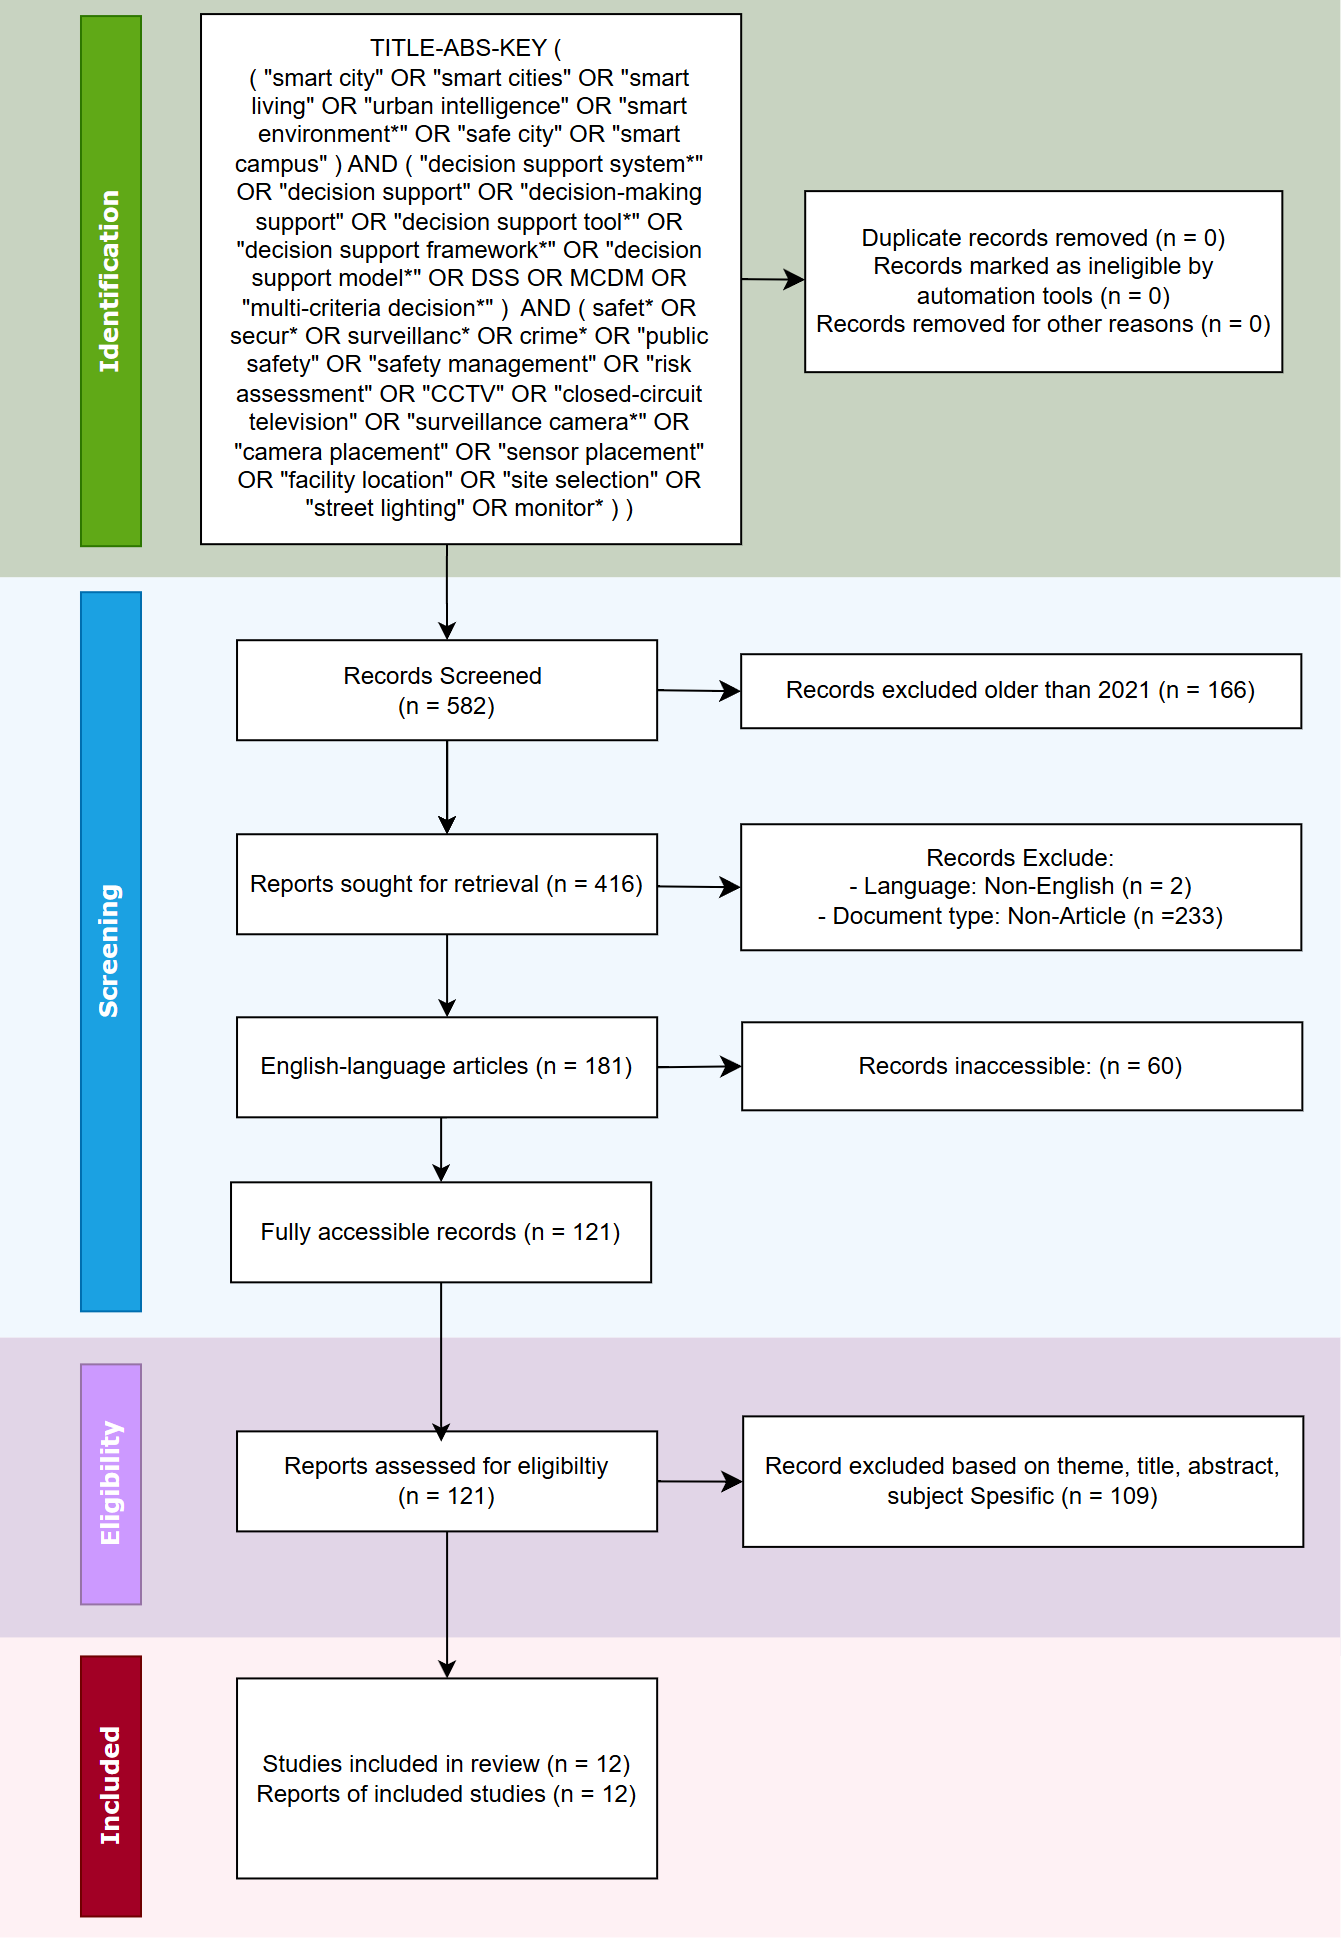
\includegraphics[width=\columnwidth]{prisma-diagram.png}
\caption{Diagram alir seleksi studi berdasarkan PRISMA-ScR (582 \textrightarrow{} 166 \textrightarrow{} 416 \textrightarrow{} 121 \textrightarrow{} 12). Tanggal pencarian: [ISI TANGGAL].}
\label{fig:prisma}
\end{figure}

\subsection{Ekstraksi dan Analisis Literatur}

Studi yang disertakan kemudian di-charting ke dalam tabel ekstraksi dengan kolom: penulis, domain permasalahan, komponen DSS, metode MCDM, kriteria utama, dan relevansi terhadap studi kasus Jatinangor. Hasil charting menjadi dasar analisis RQ1 (pemetaan arsitektur), RQ2 (sebaran metode dan taksonomi kriteria), dan penyusunan model konseptual RQ3. Sintesis dilakukan dengan pendekatan tematik, yaitu pengelompokan pola arsitektur, peran metode, dan orientasi kriteria, bukan penilaian kualitatif terhadap metode individual.

\section{HASIL DAN PEMBAHASAN}

\subsection{Analisis RQ1: Pemetaan Kerangka dan Arsitektur DSS}

\noindent\textbf{RQ1:} \textit{Bagaimana arsitektur DSS Smart Living \& Safety dipetakan dari literatur (alur input data heterogen ke engine MCDM/analitik lalu output keputusan), dan pola mana yang paling transferable terhadap keterbatasan data Jatinangor?}

\begin{table*}[!t]
\caption{Ekstraksi Literatur (Data Charting)}
\label{tab:charting}
\setlength{\tabcolsep}{3pt}
\centering
\small
\begin{tabular}{p{0.5cm}p{1.6cm}p{1.9cm}p{3.6cm}p{2.2cm}p{2.2cm}p{3.4cm}}
\toprule
\textbf{No.} & \textbf{Penulis} & \textbf{Domain} & \textbf{Komponen DSS} & \textbf{Metode MCDM} & \textbf{Kriteria Utama} & \textbf{Relevansi Jatinangor} \\
\midrule
1 & Wang et al. \cite{wang2025} & Penempatan kamera jalan, Wuwei RRT & Input simpul jalan + model coverage; engine MWVC + greedy; output titik kamera dan tiang optimal & Optimasi coverage MWVC (non-MCDM) & Coverage jalan (benefit); jumlah tiang dan kamera (cost) & Jangkar argumen anggaran (tiang 62 ke 33, kamera 196 ke 98, coverage 100\%); C4/C6/C7/C9 \\
2 & Gonzalez-Villa et al. \cite{gonzalez2024} & Counter-terrorism dan infrastruktur kritis (S4AllCities) & Input pergerakan pejalan/kendaraan + model ancaman; engine prediktif-probabilistik; output evakuasi dan rute intervensi & DSS simulasi terintegrasi (non-MCDM) & Probabilitas ancaman, egress time, estimasi korban & Pembanding arsitektur; pola simulasi ditolak untuk model UTS, dicatat sebagai varian ideal \\
3 & Feizizadeh \& Omarzadeh \cite{feizizadeh2025} & Pemetaan risiko pesepeda, Berlin & Input crowd-sensor + guna lahan; engine statistik spasial + MCDA-GIS; output peta risiko & Spatial-MCDA berbasis GIS & Volume lalu lintas, kondisi jalur, lingkungan, guna lahan, sosiodemografi & Template peta prioritas gang; C2/C5/C8 \\
4 & Ahmed et al. \cite{ahmed2022} & Smart campus, UAE & Input survei 4 kelompok pengguna; engine AHP antar-stakeholder + utility function; output tool keputusan investasi & AHP multistakeholder + utility function & Smart security and safety, navigasi kampus, adaptive learning & Skema AHP tiga kelompok; bukti safety terpenting di kawasan pendidikan; C8/C9 \\
5 & Choi et al. \cite{choi2025} & Teknologi hunian padat, Korea Selatan & Input 16 teknologi + panel 22 ahli; engine MCDM + expected utility 3 skenario; output prioritas teknologi & MCDM terintegrasi + expected utility & Importance dan utility per domain; smart safety teratas & Legitimasi fokus safety hunian padat; C5/C8 \\
6 & Kanj et al. \cite{kanj2024} & Rute barang berbahaya, smart city & Input data cloud + cost/duration/risk; engine Fuzzy AHP + Fuzzy TOPSIS; output rute teraman & Fuzzy AHP (bobot) + Fuzzy TOPSIS (ranking) & Cost, duration, risk & Justifikasi inti AHP-TOPSIS; C1/C9 \\
7 & Kabashkin et al. \cite{kabashkin2025} & Monitoring lalu lintas UAV, Astana & Input video 30 titik kritis; engine simulasi + kerangka MCDM; output evaluasi 6 skenario & MCDM evaluasi skenario berbasis simulasi & Flow, kecepatan, delay, kriteria skenario & Sampling titik kritis menjadi logika segmen gang; UAV diganti observasi manual; C2 \\
8 & Baddour et al. \cite{baddour2026} & Perencanaan diplomatic quarter & Input dataset urban publik; engine BWM + CoCoSo dengan komparasi AHP/TOPSIS/VIKOR; output ranking skenario & BWM (bobot) + CoCoSo (ranking); komparasi berangka & Security, accessibility, infrastructure, sustainability, resilience & Komparasi metode; alasan memilih AHP-TOPSIS (selisih kinerja kecil, lebih sederhana); C1/C8/C9 \\
9 & Almassawa et al. \cite{almassawa2024} & Kebijakan smart mobility, South Tangerang & Input indikator availability/security/comfort; engine PROMETHEE; output strategi kebijakan & PROMETHEE & Availability, security, comfort & Variasi metode; konteks Indonesia; C1 \\
10 & Shiddiqy et al. \cite{shiddiqy2025} & Arsitektur pertahanan IKN, Indonesia & Input dokumen kebijakan sekunder; engine SWOT + AHP; output prioritas komponen & SWOT + AHP & C4ISR, AI-surveillance, keamanan infrastruktur, kolaborasi & Bukti AHP dari data sekunder; bobot surveilans tinggi; C4/C7 \\
11 & Zheng et al. \cite{zheng2025} & Risiko banjir komunitas, Guangzhou & Input faktor alam-sosial + IoT + ArcGIS; engine DEMATEL-ISM + Bayesian Network; output risiko dan evaluasi intervensi & DEMATEL-ISM + Bayesian Network & Faktor alam dan sosial; kapasitas drainase & Logika intervensi terukur; toolchain Python + ArcGIS; C3/C9 \\
12 & Yuhang et al. \cite{yuhang2025} & Penempatan sensor grid, Guangzhou & Input proximity + kepadatan penduduk (EWM); engine BCSLP + genetic algorithm; output strategi balanced & EWM (bobot objektif) + optimasi coverage & Primary coverage, backup coverage, risiko, biaya & EWM sebagai validasi silang bobot; C4/C5/C7/C9 \\
\bottomrule
\end{tabular}
\end{table*}

Charting menunjukkan komponen DSS dapat dipetakan ke tiga lapisan umum: lapisan input (data spasial, observasi, survei pakar, data historis, citra/sensor), decision engine (MCDM, machine learning, fuzzy logic, jaringan Bayesian, simulasi, optimasi), dan decision output (peta risiko, skor, perankingan, rute, prioritas intervensi). Keberagaman domain di atas tidak diadopsi sebagai variabel fisiknya, melainkan diabstraksi menjadi pola arsitektur dan logika keputusan yang domain-agnostic.

Berdasarkan sintesis charting, arsitektur DSS pada literatur terbagi menjadi lima pola:

\begin{enumerate}
\item \textbf{GIS-MCDM dan evaluasi skenario spasial} \cite{feizizadeh2025,kabashkin2025,zheng2025}: menggabungkan lapisan spasial dengan MCDM sehingga keluaran keputusan memiliki dimensi lokasi; menjadi arsitektur utama model Jatinangor.
\item \textbf{Optimasi coverage} \cite{wang2025,yuhang2025}: memaksimalkan cakupan dengan jumlah perangkat terbatas, relevan untuk penempatan CCTV berbudget ketat.
\item \textbf{Expert-driven (survei + AHP)} \cite{ahmed2022,choi2025,baddour2026}: mengandalkan penilaian pakar dan pemangku kepentingan, sesuai data empiris terbatas.
\item \textbf{Simulasi-DSS operasional} \cite{gonzalez2024}: paling lengkap outputnya namun membutuhkan data kalibrasi berbiaya tinggi, sehingga ditolak untuk model Jatinangor.
\item \textbf{Policy-MCDA} \cite{almassawa2024,shiddiqy2025}: menghasilkan rekomendasi kebijakan terprioritas, dipakai untuk framing keluaran model.
\end{enumerate}

\begin{figure}[!t]
\centering
\begin{small}
\begin{verbatim}
Arsitektur DSS (5 pola dari 12 studi)
+-- GIS-MCDM [3][7][11]
|     -> DIPAKAI: peta prioritas spasial
+-- Optimasi coverage [1][12]
|     -> DIPAKAI: penempatan hemat alat
+-- Expert-driven [4][5][8]
|     -> DIPAKAI: bobot multistakeholder
+-- Simulasi-DSS [2]
|     -> DITOLAK: kalibrasi mahal
+-- Policy-MCDA [9][10]
       -> DIPAKAI: framing kebijakan
\end{verbatim}
\end{small}
\caption{Taksonomi lima pola arsitektur DSS dan nasibnya pada model Jatinangor.}
\label{fig:taksonomi}
\end{figure}

Penting dicatat bahwa pola hybrid (kombinasi lebih dari satu engine) dominan dalam literatur. Namun, kebutuhan data antarpola berbeda jauh: pola yang bergantung pada simulasi real-time, citra berbiaya, atau machine learning membutuhkan data berdensitas tinggi, sedangkan pola GIS-MCDM, optimasi coverage, dan expert-driven dapat berjalan di atas data tabular, data spasial statis, dan penilaian pakar. Dengan kriteria transferability, tiga pola terakhir merupakan baseline yang paling realistis untuk Jatinangor, dan kesimpulan ini menjadi dasar perancangan model pada Seksi IV.

\textbf{Jawaban RQ1:} arsitektur DSS Smart Living \& Safety dalam literatur terpetakan ke lima pola dengan alur umum input heterogen, decision engine, lalu output keputusan; pola yang paling transferable untuk Jatinangor adalah kombinasi GIS-MCDM, optimasi coverage, dan expert-driven karena ketiganya bekerja di atas data diskrit yang tersedia lokal. \textbf{Celah yang teridentifikasi:} hampir seluruh studi menguji arsitektur pada lingkungan berdata lengkap (sensor, citra, simulasi berkalibrasi), sedangkan penempatan fasilitas pengawasan pada hunian padat beranggaran terbatas dengan data diskrit praktis belum dirancang sebagai satu model utuh; celah inilah yang dijawab pada Seksi IV.

\subsection{Analisis RQ2: Sebaran Metode MCDM dan Taksonomi Kriteria}

\noindent\textbf{RQ2:} \textit{Metode MCDM apa yang digunakan dalam DSS Smart Living \& Safety, bagaimana skema pembobotan dan perankingannya diterapkan, serta bagaimana kriteria keputusan diklasifikasikan berdasarkan atribut benefit dan cost?}

\begin{table}[!t]
\caption{Sebaran dan Peran Metode MCDM}
\label{tab:metode}
\centering
\begin{tabular}{p{1.9cm}p{2.8cm}p{2.9cm}}
\toprule
\textbf{Peran} & \textbf{Metode ditemukan} & \textbf{Studi pendukung} \\
\midrule
Pembobotan subjektif (pakar) & AHP, Fuzzy AHP, BWM & \cite{ahmed2022,kanj2024,baddour2026,shiddiqy2025} \\
Pembobotan objektif (data) & Entropy Weight Method (EWM) & \cite{yuhang2025} \\
Perankingan alternatif & TOPSIS, Fuzzy TOPSIS, CoCoSo, PROMETHEE & \cite{kanj2024,baddour2026,almassawa2024} \\
Struktural/kausal & DEMATEL-ISM, Bayesian Network & \cite{zheng2025} \\
Evaluasi skenario spasial & Kerangka MCDM multi-skenario & \cite{kabashkin2025} \\
Pola pemenang (kombinasi) & AHP untuk bobot + TOPSIS untuk ranking & \cite{kanj2024} \\
\bottomrule
\end{tabular}
\end{table}

Angka frekuensi dalam tabel tidak bersifat eksklusif: satu paper dapat memakai lebih dari satu metode, sehingga jumlah kemunculan tidak dijumlahkan menjadi persentase artikel. Aturan hitung pada sintesis: hanya pemakaian sebagai engine utama yang dihitung, sedangkan komparasi metode pada \cite{baddour2026} dicatat terpisah dan bukan sebagai pemakaian. Hasilnya AHP/Fuzzy AHP dipakai primer di 3 paper \cite{ahmed2022,kanj2024,shiddiqy2025}, sedangkan BWM, EWM, TOPSIS/Fuzzy TOPSIS, CoCoSo, PROMETHEE, DEMATEL-ISM dengan Bayesian Network, dan MCDM multi-skenario masing-masing dipakai primer di 1 paper; tiga studi non-MCDM memakai optimasi MWVC \cite{wang2025}, DSS simulasi terintegrasi \cite{gonzalez2024}, dan statistik spasial \cite{feizizadeh2025}. Dari 12 studi disertakan, AHP merupakan metode yang paling sering muncul secara eksplisit dan konsisten berperan sebagai weighting method, sedangkan TOPSIS dan varian fuzzy-nya berperan sebagai ranking method. Pola kombinasi AHP lalu TOPSIS pada \cite{kanj2024} menjadi template yang paling langsung dapat diadopsi. Dua metode yang sering disebut pada rubrik kajian sejenis, yaitu SAW dan WP, tidak ditemukan secara eksplisit dalam 12 studi inti ini, sehingga tidak dijadikan dasar justifikasi model. Selain itu, komparasi berangka pada \cite{baddour2026} menunjukkan selisih kinerja antarmetode relatif kecil (agreement pakar 92,8\% untuk BWM-CoCoSo berbanding 88,6\% untuk AHP-TOPSIS, dengan selisih robustness 0,91 berbanding 0,84), sehingga kesederhanaan dan ketersediaan pakar menjadi penentu pemilihan metode, bukan perburuan skor tertinggi.

\begin{table}[!t]
\caption{Taksonomi Kriteria Keputusan}
\label{tab:taksonomi}
\centering
\begin{tabular}{p{1.2cm}p{2.0cm}p{2.4cm}p{2.0cm}}
\toprule
\textbf{Kelompok} & \textbf{Orientasi} & \textbf{Contoh dari literatur} & \textbf{Perlakuan di model} \\
\midrule
Benefit & Semakin tinggi semakin diprioritaskan (dalam konteks keputusan paper sumber) & Volume mobilitas dan aktivitas \cite{feizizadeh2025}; cakupan pengawasan \cite{wang2025,yuhang2025}; keamanan dan aksesibilitas \cite{baddour2026,almassawa2024} & Seluruh C1--C9 (skor tinggi = prioritas) \\
Cost & Semakin rendah semakin dikehendaki & Jumlah perangkat dan biaya \cite{wang2025}; risiko kecelakaan \cite{kabashkin2025}; biaya implementasi \cite{baddour2026} & Diserap ke C9 + kendala anggaran (rinci di B.3b sintesis) \\
Context-dependent & Arah preferensi tidak eksplisit pada data charting paper sumber & Faktor yang orientasinya bergantung pada formulasi model masing-masing paper (diklasifikasikan berdasarkan tujuan keputusan, bukan nama variabel) & Tidak dipaksa biner \\
\bottomrule
\end{tabular}
\end{table}

Taksonomi ini penting karena benefit dan cost merupakan sifat kriteria dalam suatu model keputusan, bukan sifat absolut dari nama variabel. Klasifikasi seluruh kriteria dilakukan terhadap tujuan keputusan paper sumber; ketika arah preferensi tidak eksplisit tercatat pada charting, kriteria dipisahkan sebagai context-dependent dan tidak dipaksa masuk biner benefit/cost. Seluruh arah kriteria pada model Jatinangor dirumuskan terhadap urgensi, yaitu skor yang lebih tinggi menandakan prioritas pemasangan yang lebih besar (Seksi IV).

\textbf{Jawaban RQ2:} metode yang muncul dalam literatur terbagi atas empat peran, yaitu pembobotan subjektif (AHP, Fuzzy AHP, BWM), pembobotan objektif (EWM), perankingan (TOPSIS, CoCoSo, PROMETHEE), dan pemodelan struktural (DEMATEL-ISM, Bayesian); pola kombinasi AHP untuk bobot lalu TOPSIS untuk peringkat adalah yang paling langsung dapat diadopsi, sedangkan kriteria keputusan terpetakan ke benefit, cost, dan context-dependent. \textbf{Celah yang teridentifikasi:} (a) komparasi bobot objektif berbasis data dengan bobot subjektif berbasis pakar jarang dilakukan dalam satu studi yang sama, (b) SAW dan WP yang lazim disebut pada kajian sejenis tidak ditemukan eksplisit pada korpus ini, sehingga tidak dapat dijadikan dasar bukti, dan (c) klasifikasi benefit/cost kerap dilakukan hanya dari nama variabel tanpa memeriksa arah preferensi di dalam formulasi model. Celah tersebut dijawab pada Seksi IV lewat skema AHP yang divalidasi silang dengan EWM serta taksonomi tiga kategori yang diterapkan konsisten.

\subsection{Sintesis RQ1 dan RQ2}

\begin{table}[!t]
\caption{Sintesis Temuan Literatur dan Implikasi}
\label{tab:sintesis}
\centering
\begin{tabular}{p{1.5cm}p{3.0cm}p{3.1cm}}
\toprule
\textbf{Aspek} & \textbf{Temuan literatur} & \textbf{Implikasi untuk Jatinangor} \\
\midrule
Arsitektur & Lima pola; hybrid dominan; kebutuhan data antarpola berbeda jauh & Pakai baseline GIS-MCDM + optimasi coverage + expert-driven \\
Input & Spasial, observasi, survei pakar, data historis, sensor/citra & Cukup data diskrit lokal: survei, OSM, rekap insiden, RAB \\
Decision engine & MCDM, ML, fuzzy, simulasi, optimasi & MCDM dipilih karena transparan dan dapat diverifikasi pakar \\
Pembobotan & Banyak berbasis pakar (AHP, BWM) & AHP tiga kelompok pemangku kepentingan (AHP primer di 3 studi) \\
Perankingan & TOPSIS, CoCoSo, PROMETHEE & TOPSIS karena ringkas dan sejalan pola pemenang \cite{kanj2024} \\
Benefit & Cakupan, aktivitas, keamanan, kepadatan & Menjadi orientasi skor C1--C9 terhadap urgensi \\
Cost & Biaya, risiko, jumlah perangkat & Diperlakukan sebagai kendala anggaran dan kriteria kelayakan \\
Context-dependent & Bergantung formulasi model & Kriteria tanpa arah eksplisit tidak dipaksa biner \\
Output & Peta risiko, skor, peringkat, prioritas & Peta prioritas segmen gang + urutan pemasangan bertahap \\
Transferability & Bergantung kebutuhan data dan kompleksitas & Kelayakan adopsi diuji pada tiga dimensi (Seksi IV-E) \\
\bottomrule
\end{tabular}
\end{table}

\section{PERANCANGAN MODEL KONSEPTUAL DSS JATINANGOR (JAWABAN RQ3)}

\noindent\textbf{RQ3:} \textit{Model konseptual DSS seperti apa yang paling layak diterapkan untuk prioritisasi CCTV di permukiman mahasiswa Jatinangor, mencakup representasi segmen gang sebagai alternatif, struktur sembilan kriteria keselamatan, skema pembobotan AHP multistakeholder dan perankingan TOPSIS, serta elemen literatur apa yang sengaja tidak diadopsi beserta alasannya?}

\subsection{Profil Lokasi dan Perumusan Alternatif}

Jatinangor dibagi menjadi beberapa desa dengan pola hunian campuran: permukiman padat berbasis indekos di sekitar gerbang kampus, koridor jalan utama yang menghubungkan simpul layanan, serta gang-gang residensial sempit dengan penerangan seadanya. Kerawanan tidak merata antarsegmen, sehingga unit keputusan yang tepat bukan desa secara keseluruhan, melainkan \textbf{segmen jalan atau gang} yang menerima satu unit CCTV.

\begin{table}[htbp]
\caption{Alternatif Segmen (A1--A5)}
\label{tab:alternatif}
\centering
\begin{tabular}{p{0.9cm}p{6.7cm}}
\toprule
\textbf{Kode} & \textbf{Segmen (contoh operasional, nama final dari observasi lapangan)} \\
\midrule
A1 & Gang kos kawasan Sayang (padat, akses sempit) \\
A2 & Ruas jalan Cikeruh dekat gerbang kampus \\
A3 & Persimpangan Hegarmanah (simpul multi-cabang) \\
A4 & Gang Cipacing (minim PJU) \\
A5 & Ruas Cileles (jalur mobilitas malam) \\
\bottomrule
\end{tabular}
\end{table}

Aturan penentuan alternatif: 4--6 segmen; setiap alternatif mewakili satu segmen yang layak menerima tepat satu unit CCTV; nama final ditetapkan berdasarkan observasi lapangan. Alternatif segmen diadopsi dari \cite{wang2025} karena unit keputusannya berupa simpul atau segmen jalan dengan coverage terukur, dan dari \cite{feizizadeh2025} karena format peta prioritas spasialnya dapat direplikasi menjadi peta prioritas gang di Jatinangor.

\subsection{Matriks Kriteria C1--C9}

Sembilan kriteria dirumuskan dengan satu arah tunggal: skor lebih tinggi berarti semakin prioritas (orientasi benefit terhadap urgensi).

\begin{table*}[!t]
\caption{Matriks Kriteria Keselamatan C1--C9}
\label{tab:kriteria}
\setlength{\tabcolsep}{4pt}
\centering
\small
\begin{tabular}{p{0.7cm}p{2.2cm}p{3.8cm}p{1.4cm}p{3.8cm}p{2.9cm}}
\toprule
\textbf{Kode} & \textbf{Kriteria} & \textbf{Definisi operasional} & \textbf{Satuan} & \textbf{Sumber data (utama / fallback)} & \textbf{Rujukan} \\
\midrule
C1 & Riwayat kerawanan segmen & Kejadian kriminalitas/kecelakaan per km per tahun & kejadian/km/th & Rekap insiden / observasi + wawancara RT & \cite{kanj2024,baddour2026,almassawa2024,feizizadeh2025} \\
C2 & Volume mobilitas malam & Orang lewat pukul 18.00--24.00 & orang/jam & Counting manual / CCTV eksisting & \cite{feizizadeh2025,kabashkin2025,almassawa2024} \\
C3 & Defisiensi penerangan & Kekurangan cahaya PJU (skor survei) & skor 1--5 & Survei malam / data dinas (fallback: observasi) & \cite{baddour2026,zheng2025} \\
C4 & Efisiensi coverage & Luas ter-cover per titik CCTV & m2/titik & Pemetaan + model coverage & \cite{wang2025,yuhang2025} \\
C5 & Kepadatan penghuni & Kamar kos per km gang & kamar/km & Pendataan kos / data desa & \cite{yuhang2025,feizizadeh2025,choi2025} \\
C6 & Derajat simpul jalan & Jumlah cabang persimpangan & cabang & OpenStreetMap + observasi & \cite{wang2025} \\
C7 & Coverage gap CCTV eksisting & Jarak ke CCTV terdekat & meter & Survei titik CCTV & \cite{wang2025,yuhang2025} \\
C8 & Kedekatan guna lahan rentan & Radius 150 m ke kos, ATM, warung 24 jam, gerbang kampus & unit & Observasi + POI & \cite{feizizadeh2025,baddour2026,ahmed2022} \\
C9 & Kelayakan implementasi & Kesiapan tiang/listrik/internet dikurangi estimasi biaya & skor & Survei jaringan + RAB & \cite{kanj2024,wang2025,baddour2026} \\
\bottomrule
\end{tabular}
\end{table*}

\textbf{Validasi rujukan kriteria:} C1 didukung \cite{kanj2024,baddour2026,almassawa2024}; C2 oleh \cite{feizizadeh2025,kabashkin2025,almassawa2024}; C3 oleh \cite{baddour2026,zheng2025}; C4 oleh \cite{wang2025,yuhang2025}; C5 oleh \cite{yuhang2025,feizizadeh2025,choi2025}; C7 oleh \cite{wang2025,yuhang2025}; C8 oleh \cite{feizizadeh2025,baddour2026,ahmed2022}; dan C9 oleh \cite{kanj2024,wang2025,baddour2026}. Delapan dari sembilan kriteria ditelusuri ke minimal dua studi. C6 (derajat simpul jalan) hanya didukung eksplisit oleh \cite{wang2025} yang menjadikan adjacency degree sebagai bobot vertex utama; keterbatasan satu rujukan ini dicatat apa adanya, dengan penguatan tidak langsung dari pola struktur jaringan pada \cite{yuhang2025}.

\textbf{Urutan prioritas kriteria:} berdasarkan frekuensi dukungan di 12 studi, dengan seri yang diputus menurut relevansi langsung terhadap keputusan penempatan CCTV (kendala anggaran dan paparan didahulukan atas faktor pendukung), urutannya adalah C1 $>$ C9 $>$ C2 $>$ C5 $>$ C8 $>$ C4 $>$ C7 $>$ C3 $>$ C6. C1 menempati urutan pertama dengan dukungan 4 studi sebagai inti urgensi pemasangan; C9 kedua sebagai jangkar kelayakan anggaran \cite{wang2025}; C6 terakhir karena bersumber tunggal.

\subsection{Skema Pembobotan AHP dan Perankingan TOPSIS}

\textbf{Pembobotan AHP multistakeholder} mengadopsi skema AHP lintas kelompok dari \cite{ahmed2022} karena studi itu membuktikan AHP dapat mempertemukan persepsi empat kelompok pengguna dalam satu bobot konsensus, dengan angka acuan konsistensi dan komparasi dari \cite{baddour2026} dan \cite{shiddiqy2025} yang keduanya menunjukkan AHP berjalan valid bahkan dengan data sekunder:

\begin{enumerate}
\item Responden tiga kelompok: (a) pemerintah daerah (dinas terkait, kecamatan), (b) kampus dan pengelola kawasan, (c) warga (RT, pemilik kos).
\item Kuesioner pairwise comparison sembilan kriteria per kelompok dengan skala Saaty 1--9.
\item Agregasi antarkelompok menggunakan geometric mean; uji Consistency Ratio dengan ambang CR $<$ 0,1 \textbf{[FULLTEXT-VERIFY: angka acuan CR 0,046 dari \cite{baddour2026}]}, dihitung lewat lamda-maks, CI = (lamda-maks $-$ n)/(n $-$ 1), dan CR = CI/RI dengan RI untuk n = 9 sebesar 1,45.
\item Validasi silang opsional: bobot objektif Entropy Weight Method dari data lapangan \cite{yuhang2025} sebagai pembanding terhadap bobot subjektif AHP; selisih besar memicu diskusi ulang dengan pakar, bukan penggantian otomatis.
\end{enumerate}

\textbf{Perankingan TOPSIS} mengadopsi pola pemenang AHP-TOPSIS dari \cite{kanj2024} karena kombinasi itu terbukti menyelesaikan perankingan multi-kriteria dengan kriteria ringkas tanpa infrastruktur komputasi berat:

\begin{enumerate}
\item Matriks keputusan A1--A5 terhadap C1--C9 dari data lapangan.
\item Normalisasi kolom matriks lalu pengalikan bobot AHP menjadi matriks terbobot.
\item Perhitungan jarak tiap alternatif ke solusi ideal positif dan negatif, lalu closeness coefficient $C(i) = D-(i)/(D+(i) + D-(i))$ untuk menetapkan peringkat prioritas pemasangan dari nilai terbesar.
\item Analisis sensitivitas bobot sebesar $\pm$20\% untuk menguji ketahanan peringkat, mengikuti praktik sensitivitas pada \cite{baddour2026}; peringkat dinyatakan robust bila posisinya tidak berubah.
\end{enumerate}

Justifikasi teoritis pemilihan metode: dari kandidat metode pembobotan dan perankingan yang lazim (SAW, WP, TOPSIS, AHP), kombinasi AHP-TOPSIS yang dipilih karena (a) terbukti dipakai berpasangan dalam literatur korpus ini \cite{kanj2024}, (b) AHP mengakomodasi penilaian pakar secara konsisten, sesuai ketersediaan data Jatinangor, sebagaimana dibuktikan AHP berjalan dari data sekunder pada \cite{shiddiqy2025}, (c) TOPSIS ringkas, transparan, dan menangani kompromi benefit-cost secara langsung, sementara selisih kinerja terhadap metode lebih kompleks ternyata kecil menurut komparasi berangka \cite{baddour2026}, dan (d) SAW dan WP tidak ditemukan eksplisit pada 12 studi inti, sehingga tidak memiliki dukungan bukti dalam protokol ini.

\subsection{Arsitektur Konseptual dan Justifikasi Adopsi}

\begin{figure*}[!t]
\centering
\begin{small}
\begin{verbatim}
INPUT LAYER (data diskrit lokal)
  C1 rekap insiden | C2 counting manual | C3 survei penerangan
  C4/C6/C7 pemetaan OSM + coverage | C5 data kos | C8 POI | C9 RAB
        |
        v
PREPROCESSING
  pembersihan data | kodifikasi segmen A1-A5 | normalisasi kriteria
        |
        v
DECISION ENGINE
  [AHP] bobot C1-C9 per kelompok -> agregasi geometric mean + CR
  [TOPSIS] matriks keputusan -> normalisasi -> closeness -> ranking
  [GIS] pemetaan segmen + gap coverage -> visualisasi peta
        |
        v
DECISION OUTPUT
  peringkat prioritas A1-A5 | peta prioritas segmen gang
  | urutan pemasangan bertahap sesuai anggaran
\end{verbatim}
\end{small}
\caption{Arsitektur konseptual empat lapisan DSS prioritas CCTV Jatinangor.}
\label{fig:arsitektur}
\end{figure*}

Arsitektur empat lapisan pada Gambar~\ref{fig:arsitektur} mengadopsi pola GIS-MCDM dari \cite{feizizadeh2025} dan \cite{kabashkin2025} karena keduanya membuktikan keluaran keputusan spasial terbangun dari data lintas sumber, logika optimasi coverage dari \cite{wang2025} dan \cite{yuhang2025} karena keduanya menunjukkan cakupan penuh tercapai dengan jumlah perangkat jauh lebih sedikit, serta skema expert-driven dari \cite{ahmed2022} dan \cite{baddour2026} karena penilaian pakar adalah sumber bobot yang paling tersedia di Jatinangor. Justifikasi adopsi dan penolakan elemen literatur dicatat eksplisit:

\begin{itemize}
\item \textbf{Ditolak: simulasi-DSS operasional ala \cite{gonzalez2024}} karena membutuhkan data kalibrasi berbiaya tinggi dan infrastruktur yang tidak tersedia di Jatinangor.
\item \textbf{Ditolak: kombinasi BWM-CoCoSo ala \cite{baddour2026}} karena selisih kinerja terhadap AHP-TOPSIS kecil, sedangkan pakar tersedia untuk AHP dan prosesnya lebih mudah diaudit.
\item \textbf{Ditunda: metrik response time dan egress ala \cite{gonzalez2024}} karena datanya tidak tersedia; dicatat sebagai keterbatasan dan arah riset lanjutan.
\item \textbf{Dicatat sebagai catatan disiplin protokol:} template terkait AHP-GIS-Fuzzy-TOPSIS yang relevan namun terbit 2020 gugur pada aturan tahun 2021--2026.
\end{itemize}

\subsection{Kelayakan Adopsi Model}

Kelayakan model diuji pada tiga dimensi. \textbf{Pertama, kebutuhan data:} seluruh input berupa data diskrit non-streaming (rekap insiden, counting manual, survei, OSM, RAB) sehingga tidak bergantung pada jaringan sensor kontinu maupun langganan citra berbiaya. \textbf{Kedua, kompleksitas metode:} AHP dan TOPSIS transparan, dapat dihitung manual maupun lembar kerja, dan tidak menuntut infrastruktur komputasi berat; CR dan analisis sensitivitas menyediakan uji kualitas yang jelas. \textbf{Ketiga, keluaran:} model menghasilkan peringkat, peta prioritas, dan urutan pemasangan yang langsung dapat dipakai sebagai dasar pengalokasian anggaran bertahap. Dengan tiga dimensi tersebut, model dapat dijalankan oleh pemangku kepentingan lokal dengan data yang tersedia, dan hanya kehilangan akurasi terbaiknya ketika data lapangan belum lengkap, bukan ketika sistem gagal dioperasikan.

\section{KESIMPULAN DAN ROADMAP SOFTWARE}

Kajian ini memetakan 12 studi literatur melalui protokol PRISMA-ScR dan menemukan lima pola arsitektur DSS keselamatan perkotaan, sebaran metode MCDM dengan pola dominan AHP untuk pembobotan dan TOPSIS untuk perankingan, serta taksonomi kriteria benefit, cost, dan context-dependent. Dari sintesis tersebut dirancang model konseptual DSS prioritisasi CCTV untuk Jatinangor: alternatif segmen gang A1--A5, matriks kriteria C1--C9 dengan satu arah terhadap urgensi dan urutan prioritas C1$>$C9$>$C2$>$C5$>$C8$>$C4$>$C7$>$C3$>$C6, pembobotan AHP tiga kelompok pemangku kepentingan, perankingan TOPSIS dengan analisis sensitivitas, dan arsitektur empat lapisan berbasis data diskrit.

Roadmap pengembangan menuju perangkat lunak pasca-UTS:

\begin{enumerate}
\item \textbf{Pengumpulan data lapangan:} observasi segmen A1--A5, counting mobilitas malam, survei penerangan, pendataan CCTV eksisting, dan RAB sebagai input matriks keputusan.
\item \textbf{Prototipe dasbor:} perhitungan AHP-TOPSIS diimplementasikan dalam skrip atau lembar kerja terhitung, disertai visualisasi peta prioritas segmen berbasis GIS ringan.
\item \textbf{Validasi pakar:} pengujian matriks pairwise comparison bersama pemangku kepentingan untuk mengkalibrasi bobot dan konsistensi.
\item \textbf{Skala lanjut (UAS):} penambahan sumber data dinamis, integrasi kanal aduan warga, dan varian pemantauan real-time yang selama ini ditunda.
\end{enumerate}

Keterbatasan kajian meliputi: verifikasi teks lengkap pada sebagian klaim menunggu dokumen full-text; pencarian terbatas pada satu database (Scopus) berbahasa Inggris; rentang tahun 2021--2026; serta seluruh nilai kriteria dan bobot dalam model masih berupa skema yang menunggu data lapangan.

\section*{Deklarasi Penggunaan Generative AI}

[Diisi tim: alat yang digunakan (opencode/Gemini) dan perannya (bantuan screening awal, draf charting, draf tulisan, format); verifikasi data, keputusan seleksi, dan penyusunan final seluruhnya oleh anggota tim.]

\begin{thebibliography}{12}
\bibitem{wang2025} L. Wang, Y. Zhang, T. Feng, and X. Qi, ``Monitoring layout and optimisation method based on minimum weighted vertices of roads,'' \emph{Applied Sciences}, vol. 15, no. 21, 2025, doi: 10.3390/app152111622.
\bibitem{gonzalez2024} J. Gonz\'{a}lez-Villa \emph{et al.}, ``Decision-support system for safety and security assessment and management in smart cities,'' \emph{Multimedia Tools and Applications}, vol. 83, no. 22, pp. 61971--61994, 2024, doi: 10.1007/s11042-023-16020-6.
\bibitem{feizizadeh2025} B. Feizizadeh and D. Omarzadeh, ``A GIS based spatiotemporal modelling approach for cycling risk mapping using crowd-sourced sensor data,'' \emph{Annals of GIS}, vol. 31, no. 2, pp. 333--351, 2025, doi: 10.1080/19475683.2025.2453550.
\bibitem{ahmed2022} V. Ahmed \emph{et al.}, ``A multi-attribute utility decision support tool for a smart campus---UAE as a case study,'' \emph{Frontiers in Built Environment}, vol. 8, 2022, doi: 10.3389/fbuil.2022.1044646.
\bibitem{choi2025} J. Choi, J. Ok, and I. Yu, ``Smart city technologies for apartment complexes in South Korea: expert prioritization and expected utility evaluation,'' \emph{J. Asian Architecture and Building Engineering}, 2025, doi: 10.1080/13467581.2025.2605740.
\bibitem{kanj2024} H. Kanj \emph{et al.}, ``Dynamic decision making process for dangerous good transportation using a combination of TOPSIS and AHP methods with fuzzy sets,'' \emph{IEEE Access}, vol. 12, pp. 40450--40479, 2024, doi: 10.1109/ACCESS.2024.3372852.
\bibitem{kabashkin2025} I. Kabashkin \emph{et al.}, ``Synchronized multi-point UAV-based traffic monitoring for urban infrastructure decision support,'' \emph{Drones}, vol. 9, no. 5, 2025, doi: 10.3390/drones9050370.
\bibitem{baddour2026} O. Baddour, A. Bhogayata, and T. Vora, ``Intelligent decision support for diplomatic quarter planning through multi-criteria analysis and urban intelligence,'' \emph{J. Intelligent Decision Making and Information Science}, vol. 3, no. 3S, pp. 1612--1629, 2026, doi: 10.59543/jidmis.v3.958.
\bibitem{almassawa2024} S. F. Almassawa \emph{et al.}, ``Policy on the implementation of smart mobility in South Tangerang City, Indonesia based on public transportation using the PROMETHEE method,'' \emph{Planning Malaysia}, vol. 22, no. 5, pp. 293--306, 2024, doi: 10.21837/pm.v22i34.1590.
\bibitem{shiddiqy2025} M. A. A. Shiddiqy \emph{et al.}, ``An integrated smart defense architecture for the Nusantara capital city of Indonesia,'' \emph{Int. J. Safety and Security Engineering}, vol. 15, no. 12, pp. 2561--2572, 2025, doi: 10.18280/ijsse.151213.
\bibitem{zheng2025} X. Zheng, K. Wang, and M. Liu, ``A Bayesian Network and DEMATEL-ISM approach for smart community flood risk assessment: a case study of Tangxia, China,'' \emph{J. Cases on Information Technology}, vol. 27, no. 1, 2025, doi: 10.4018/JCIT.386165.
\bibitem{yuhang2025} E. Yuhang \emph{et al.}, ``Sensor placement optimization for power grid condition monitoring based on a backup coverage model: a case study of Guangzhou,'' \emph{Applied Sciences}, vol. 15, no. 23, 2025, doi: 10.3390/app152312570.
\end{thebibliography}

\color{red}
IEEE conference templates contain guidance text for composing and formatting conference papers. Please ensure that all template text is removed from your conference paper prior to submission to the conference. Failure to remove the template text from your paper may result in your paper not being published.

\end{document}
